\chapter{Simulaci\'on y caracterizaci\'on de la emisi\'on de radio en eventos ES}
\label{ch:simulacionRadio}

Tal como se describi\'o en el cap\'itulo \ref{ch:easRadio}, la emisi\'on de radio de las lluvias atmosf\'ericas extendidas conforman un fen\'omeno s\'umamente complicado, cuyo c\'alculo se aborda usualmente mediante modelos efectivos o simulaciones de Monte Carlo.
En particular, en esta tesis se opt\'o por el segundo tratamiento, lo que permiti\'o utilizar la experiencia adquirida al calcular la exposici\'on de Auger a este nuevo c\'omputo.

En la primer parte de este cap\'itulo se describe la cadena de simulaciones utilizada para calcular la se\~nal esperada sobre un arreglo de antenas de radio al detectar neutrinos ES, necesarias para realizar el c\'alculo de exposici\'on.
En particular, se exponen los detalles m\'as relevantes del algoritmo de c\'alculo de la se\~nal utilizado por \zhs{}, la extensi\'on de \aires{} utilizada para simular la emisi\'on de radio de las EAS.

En la segunda parte se realiza una caracterizaci\'on de la huella de campo el\'ectrico dejada por lluvias atmosf\'ericas iniciadas por neutrinos ES.

\section{Simulaci\'on de la se\~nal}
\label{sc:simRadio}
	
	Como ya se describi\'o en el cap\'itulo \ref{ch:simulacionAuger}, la simulaci\'on de la se\~nal de eventos ES consta de tres etapas: la simulaci\'on de la interacci\'on primaria, el desarrollo de la EAS, que esta vez incluye la emisi\'on de radio y el c\'omputo de la se\~nal sobre el detector.
	\begin{description}
	\item[Interacción primaria:] Al igual que en la primer parte de esta tesis, la interacci\'on neutrino nucleon se proces\'o utilizando \tauola{}, que se describe en la secci\'on \ref{sbsc:tauola}.
	\item[Desarrollo de la EAS:] como se discuti\'o en la secci\'on \ref{sc:gen_emision} la emisi\'on de radio de una EAS puede conseguirse superponiendo la generada por cada particula de la lluvia. Por este motivo, para obtener el campo el\'ectrico a nivel del suelo se utiliz\'o el programa \zhs{}, una modificaci\'on de \aires{} que incluye el c\'alculo requerido. La descripci\'on de \zhs{} se realiza en la secci\'on \ref{sbsc:zhaires}.
	\item[Señal en el detector:] La salida de \zhs{} consiste en el campo el\'ectrico en funci\'on del tiempo sobre una lista de observadores (antenas) ubicados en posici\'ones prefijadas. Para transformar esta se\~nal cruda en la obtenida por una antena real es necesario aplicar una serie de algoritmos, que se describen en la secci\'on \ref{XXX}.
	\end{description}
	
	
	\subsection{ZHAireS}
	\label{sbsc:zhaires}

	\zhs{} es una implementaci\'on del las rutinas de ZHS \cite{1_halzen_zas_stanev_1991,2_zas_halzen_stanev_1992} sobre \aires{} desarrollada por Jaime Alvarez-Muñiz, Washington Rodriguez-Carvhalo Jr. y Matias Tueros en el Departamento de Física de Partículas Universidad de Santiago de Compostela, España.
	\zhs{}, conserva todas las capacidades de \aires{} y agrega la posibilidad de simular el la emisi\'on de radio de la EAS, incluyendo nuevas directivas de entrada que permiten controlar con buen detalle la simulación.

		\subsubsection{C\'omputo de la se\~nal}
		
		La metodolog\'ia aplicada en \zhs{} para calcular la se\~nal es simple: cada vez que el algoritmo de \aires{} avanza una part\'icula se llama a las rutinas de ZHS.
		Estas calculan el pulso electromagn\'etico que la partícula generar\'ia en ciertos observadores (o antenas) que se ubican en posiciones predefinidas, lo que se esquematiza en la figura \ref{fig:trackSch}.
		%
		\begin{figure}[ht!]
		\centering
			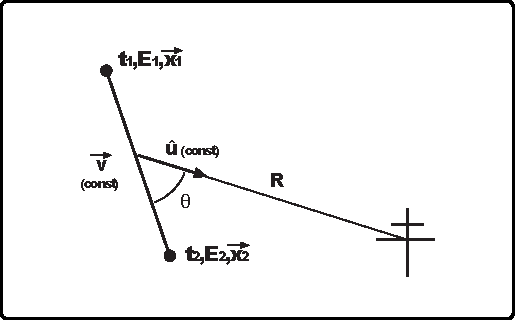
\includegraphics[width=0.6\textwidth]{fig/simulacionRadio/trackSch}
			\caption{\label{fig:trackSch} Esquema del track que avanza una par\'icula al ser simulada por \aires{}.}
		\end{figure}
		
		El c\'alculo exacto de la emisi\'on electromagn\'etica de una part\'icula que se desplaza con velocidad constante en cierto camino involucra la resoluci\'on num\'erica de integrales.
		Esto se vuelve impracticable computacionalmente si se tiene en cuenta que una lluvia típica de \cant{1}{EeV} puede implicar la simulación de $10^{10}$ partículas.
		Las rutinas de ZHS utilizan una aproximaci\'on que salva este problema a costa de cumplir las siguientes hip\'otesis:
		\begin{enumerate}
		\item El observador se encuentra en la zona de campo lejano
		\begin{equation}
		kr\gg1
		\end{equation}
		\item La longitud del track es peque\~na a comparaci\'on de la distancia al observador, $\eta\ll1$, con
		\begin{equation}
		\eta = \frac{k L^2}{R}\sin^2\theta
		\end{equation}
		donde $L\equiv v(t_1-t_2)$ es la longitud del track.
		\item La inversa distancia entre cualquier punto del track y el observador debe poder ser considerada una constante
		\begin{equation}
		\frac{1}{r(t)}\sim\frac{1}{R}
		\end{equation}
		\end{enumerate}
		%
		Si el tama\~no de los tracks obtenidos a partir del algoritmo de \aires{} no siatisface alguna de las condiciones 2 o 3, una rutina se encarga de partirlo en trozos lo suficientemente chicos como para que suceda.
		Si no se llegara a cumplir la condici\'on n\'umero 1, ser\'ia necesario utilizar la soluci\'on exacta del problema, lo que no se encuentra implementado en \zhs{} hasta el momento.
		Esta es una limitaci\'on conocida del c\'odigo, que genera se\~nales artificiales en las antenas. Afortunadamente, la probabilidad de que esto ocurra es muy baja incluso en EAS que se desarrollan muy cerca del detector como las iniciadas por neutrinos ES.
		
		Una vez que los tracks cumplen las condiciones necesarias, se calcula el potencial vector $\vec{A}(t,\hat{u})$ y el campo el\'ectrico $\vec{E}(t,\hat{u})$ en la posici\'on del observador utilizando las ecuaciones \ref{eq:afield} y \ref{eq:efield}.
		\begin{equation}
		\vec{A}(t,\hat{u})
		=
		\frac{\mu e}{4\pi Rc}
		\vec\beta_{\bot}
		\frac{\Theta(t-t^{det}_1)-\Theta(t-t^{det}_2)}{1-n\vec\beta\cdot\hat u}
		\label{eq:afield}
		\end{equation}
	% 	$\vec E(t)=-\partial\vec{A}/\partial t $
		\begin{equation}
		\vec{E}(t,\hat{u})
		=
		-\frac{\mu e}{4\pi Rc}
		\vec\beta_{\bot}
		\frac{\delta(t-t^{det}_1)-\delta(t-t^{det}_2)}{1-n\vec\beta\cdot\hat u}
		\label{eq:efield}
		\end{equation}
		En estas, como en la figura \ref{fig:trackSch}, $\hat{u}$ es el versor que indica la direcci\'on entre la mitad del track y el observador, $\vec\beta=\vec v/c$, $\vec\beta_{\bot}=-[\hat{u}\times(\hat{u}\times\vec\beta)]$ es la proyecci\'on de $\vec\beta$ sobre el plano perpendicular a $\hat u$ y $t_{1,2}^{det}=t_{1,2}+nR/c-n\vec\beta \cdot \hat u (t_{1,2}-t_0)$ son los tiempos de detecci\'on del principio y final del track respectivamente, con $t_0=(t_1+t_2)/2$. Por otro lado, $\Theta(x)$ y $\delta(x)$ son las funciones escalón de Heaviside y delta de Dirac respectivamente.
		
		Para realizar un c\'alculo correcto del tiempo de arrivo de la se\~nal a la antena, es necesario tener un modelo que describa el \'indice de refracci\'on de la atm\'osfera.
		La implementación del mismo en \zhs{} se realiza como en la ecuaci\'on \ref{eq:refIndexEff}.
		%
		\begin{equation}
			\begin{matrix}
			n_{eff}
			=
			1+{\mathcal R}_{eff}\times10^{-6}
			&
			{\rm con}
			&
			{\mathcal R}_{eff}
			=
			\frac{1}{R}\int_0^R{\mathcal R}(h)dl
			\end{matrix}
		\label{eq:refIndexEff}
		\end{equation}
		%
		En esta, ${\mathcal R}(h) = \left[ n(h)-1 \right] \times 10^6$.
		Para ${\mathcal R}(h)$, \zhs{} ofrece la posibilidad de utilizar un valor constante, o un modelo exponencial como el de la ecuaci\'on \ref{eq:refIndexExp} en el que es posible fijar su valor a nivel del suelo.
		\begin{equation}
		{\mathcal R}(h)
		=
		{\mathcal R}_o
		\exp{-K_rh}
		\label{eq:refIndexExp}
		\end{equation}
		Los valores por default son ${\mathcal R}_o={\mathcal R}(h=0)\equiv 325$ y $K_r=0.1218km^{-1}$.
		Con estos valores es posible reproducir los valores calculados en \cite{gerson1948polar} con un $1\%$ precisi\'on hasta una altura de \cant{20}{km}.
		A mayor altitud la aproximaci\'on exponencial para ${\mathcal R}$ sobreestima el \'indice de refracci\'on, pero m\'as all\'a de los \cant{20}{km} la lluvia recien ha comenzado a desarrollarse, por lo que la cantidad de part\'iculas es relativamente peque\~na por lo que esta zona contribuye muy poco a la se\~nal total.
		
		Otro factor a tener en cuenta es que cuando las lluvia a simular es muy inclinada, la altura que se utiliza en la ecuaci\'on \ref{eq:refIndexExp} debe ser medida desde la superficie de la tierra, sin utilizar la aproximai\'on de tierra plana, como se muestra en la figura \ref{fig:refIndex}.
		\begin{figure}[ht!]
		\centering
			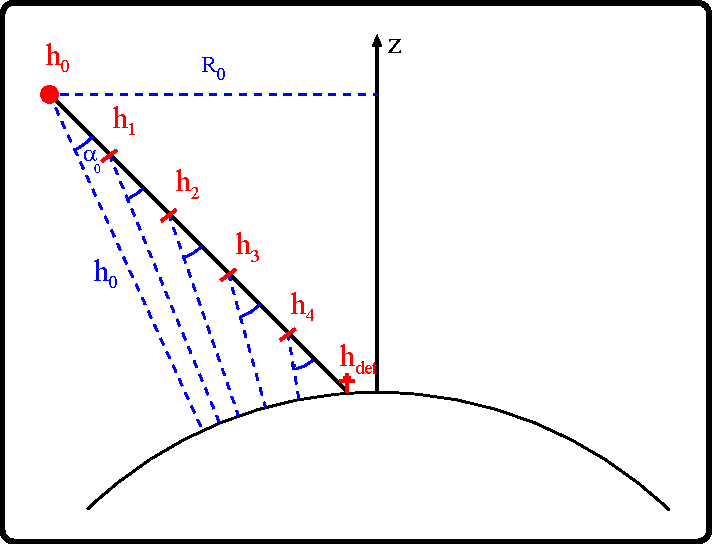
\includegraphics[width=0.6\textwidth]{fig/simulacionRadio/refIndex}
			\caption{\label{fig:refIndex} Esquema del m\'etodo mediante el que se tiene en cuenta la curvatura de la tierra al momento de calcular el \'indice de refracci\'on de la atm\'osfera para diferentes alturas.}
		\end{figure}
		Dado que realizar la integral descripta en \ref{eq:refIndexEff} en estas condiciones es muy costoso, se discretiza $R$ en un n\'umero finito de tramos y supone el \'indice de refracci\'on constrante en cada uno de ellos.
		
		Una vez calculadas las amplitudes de los campos y los tiempos de arrivo de las se\~nales debidas a cada track, el campo total en cada observador se guarda utilizando bines temporales prefijados, como la ecuaci\'on \ref{eq:eAntField}, donde el \'indice $j$ corre sobre las part\'iculas simuladas y $\omega_j$ es el peso estad\'istico que pose\'ia la part\'icula que emiti\'o el campo $\vec{E}_j$.
		\begin{equation}
		\vec{E}(t_i)=\sum_{j:t_j\varepsilon[t_i,t_{i+1}]}\vec{E}_j(t_j)\omega_j
		\label{eq:eAntField}
		\end{equation}
		%
		La ecuaci\'on \ref{eq:eAntField} muestra claramente que la se\~nal simulada en una dada antena depende fuertemente del algoritmo de thinning utilizado. 
		
		Dado que la mayor contribuci\'on al campo el\'ectrico proviene de las part\'iculas de media y baja energ\'ia, es poco deseable la aparici\'on de partículas con peso extremadamente alto.
		En consecuencia y como bajar el nivel de thinning es poco eficiente, en la simulación se utiliza un \emph{weight factor} peque\~no.

		\subsubsection{Dificultades técnicas}

		Intentando no volver esta sección tediosa se pretende enumerar una serie de dificultades técnicas a la hora de simular la señal de radio emitida por neutrinos ES utilizando \zhs{}.

		En primer lugar, al igual que en las simulaciones realizadas para Auger es necesario utilizar los productos de decaimiento generados con \tauola{} y luego inyectarlos en \aires{} con las posiciones y velocidades correctas.

		Luego, la mayor dificultad técnica resulta de la gran cantidad de tiempo de máquina que requiere realizar la simulación de la emisión de radio.
		Para contextualizar la situación, una simulación típica puede implicar la necesidad de conocer la señal en algunos cientos de observadores.
		Dado que cada vez que se avanza una partícula es necesario calcular la señal en cada uno de ellos, luego de la primer decena el tiempo de simulación depende casi linealmente de su numero, es decir, se torna despreciable el tiempo que toma simular la evolución de la lluvia.
		Con todo esto, como la simulación de una lluvia de \cant{10^{18}}{eV} puede tomar del orden de algunas horas por decena de anteas\footnote{Este número depende fuertemente del nivel de thinning elegido}, la simulación completa de cada lluvia puede requerir del orden del centenar de horas de tiempo de CPU.
		La única manera de salvar este inconveniente es partiendo el detector en grupos mas pequeños de antenas, de entre 10 y 40, donde es necesario tener la precaución de que la evolución de la lluvia se simule con la misma semilla en cada vez.

	
\section{Tratamiento de la se\~nal}
	
	- Descripcion de la antena: pag 26 harm thesis
	
	
	\subsubsection{Señal en la antena}
	La figura \ref{fig:antSig} se grafican las componentes del campo eléctrico en una antena a nivel del suelo y su espectro. La misma se encuentra ubicada sobre el punto de impacto del cono \cher{}.
	%
	\begin{figure}[ht!]
		\centering
		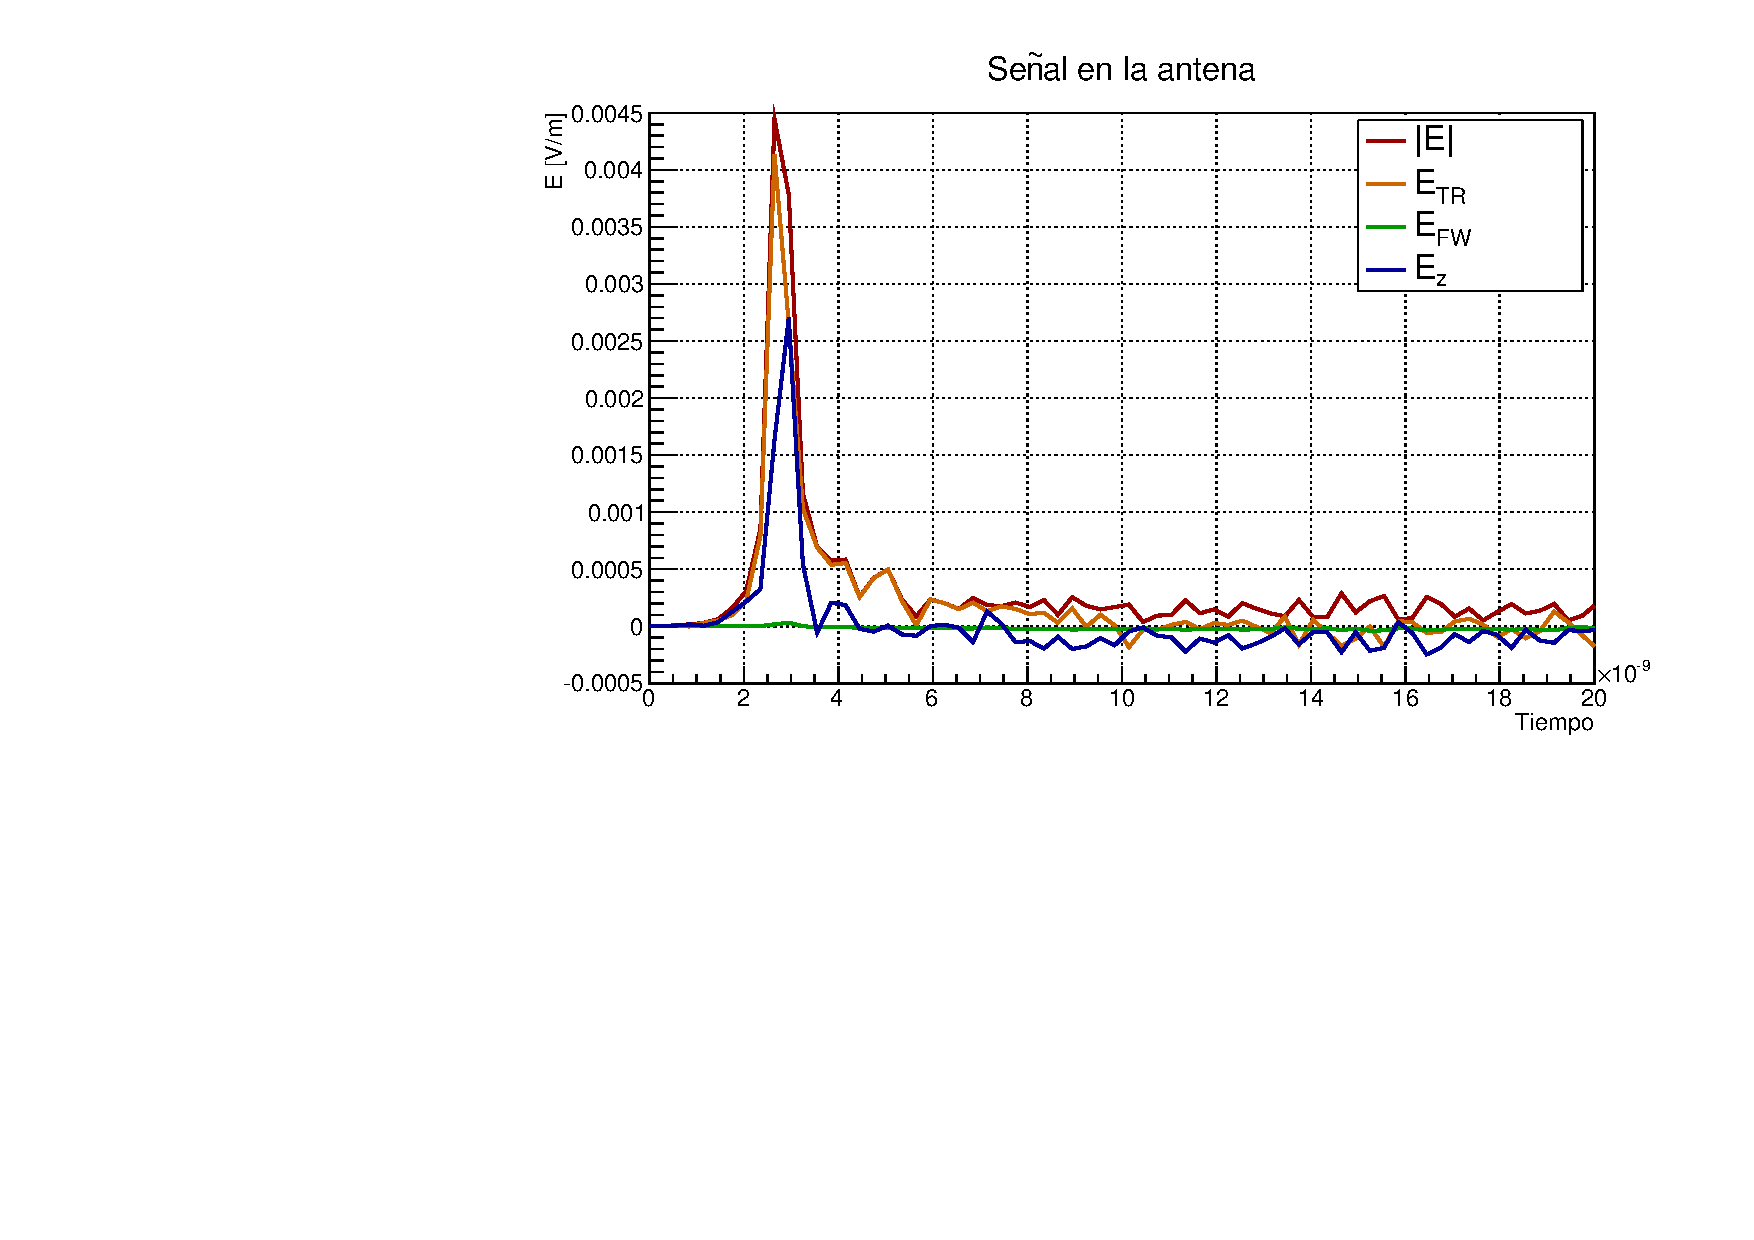
\includegraphics[width=0.8\textwidth]{./fig/simulacionRadio/antennaSignal}\\
		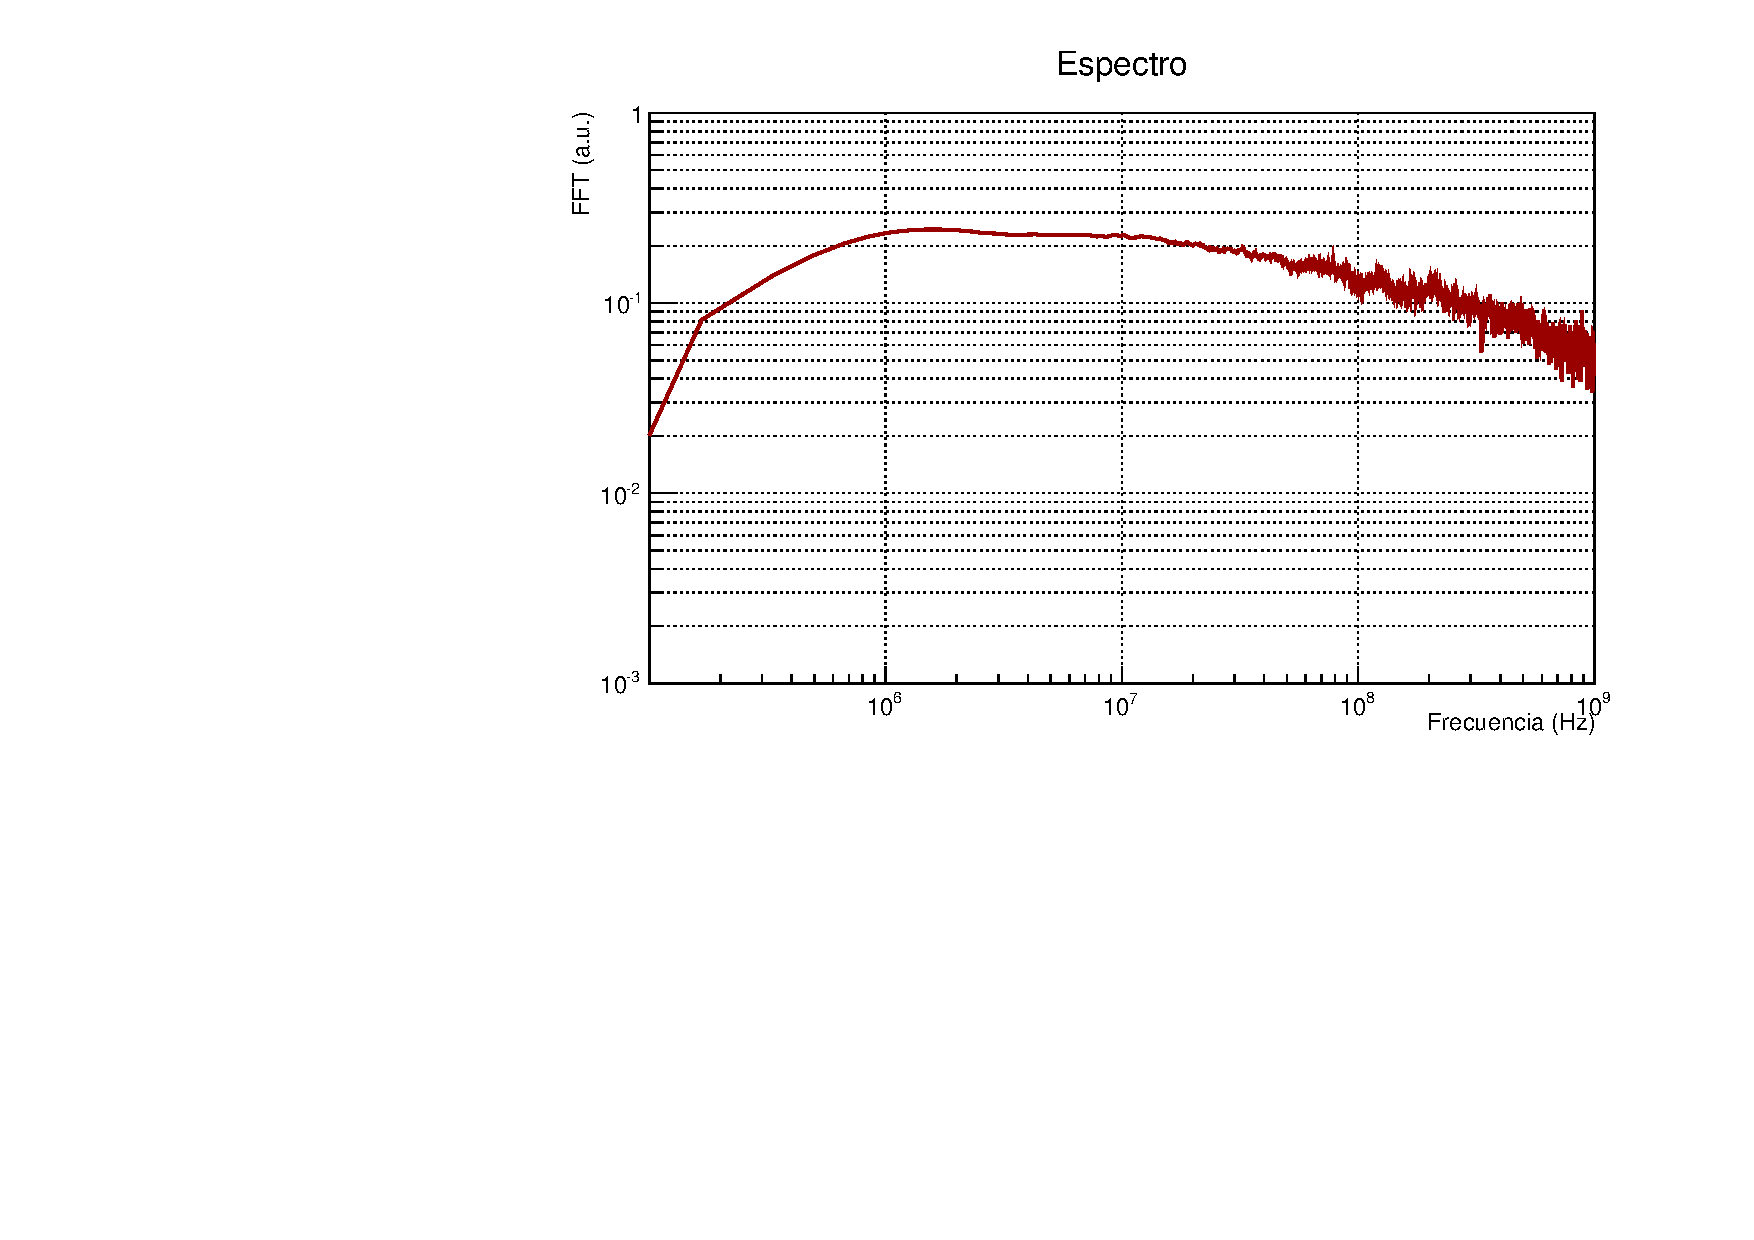
\includegraphics[width=0.8\textwidth]{./fig/simulacionRadio/antennaSpec}
		\caption{\label{fig:antSig}
		Arriba: se observa la señal en una antena colocada a nivel del suelo, ubicada sobre el cono \cher{}. Según lo expuesto en la seccción \ref{ch:easRadio}, el pico de señal correspondiente a la emisión coherente del máximo de la lluvia.
		Abajo: transformada de Fourier de la señal de la antena. Se observa coherencia hasta frecuencias casi del $\rm GHz$.
		}
	\end{figure}
	%
	Como se expuso en la sección \ref{ch:easRadio}, el pico observado en la señal corresponde a la emisión coherente de las partículas generadas en el máximo de la lluvia por lo que su espectro muestra coherencia hasta frecuencias casi del $\rm GHz$.
	Es importante destacar que esta señal se encuentra a un nivel que puede ser detectado por sobre le nivel del ruido. 
	
	Una vez obtenido el campo eléctrico en cada antena del detector es necesario simular su respuesta.
	Para ello en este trabajo se considera la posibilidad mas simple de todas
	
	
	\begin{figure}[ht!]
		\centering
		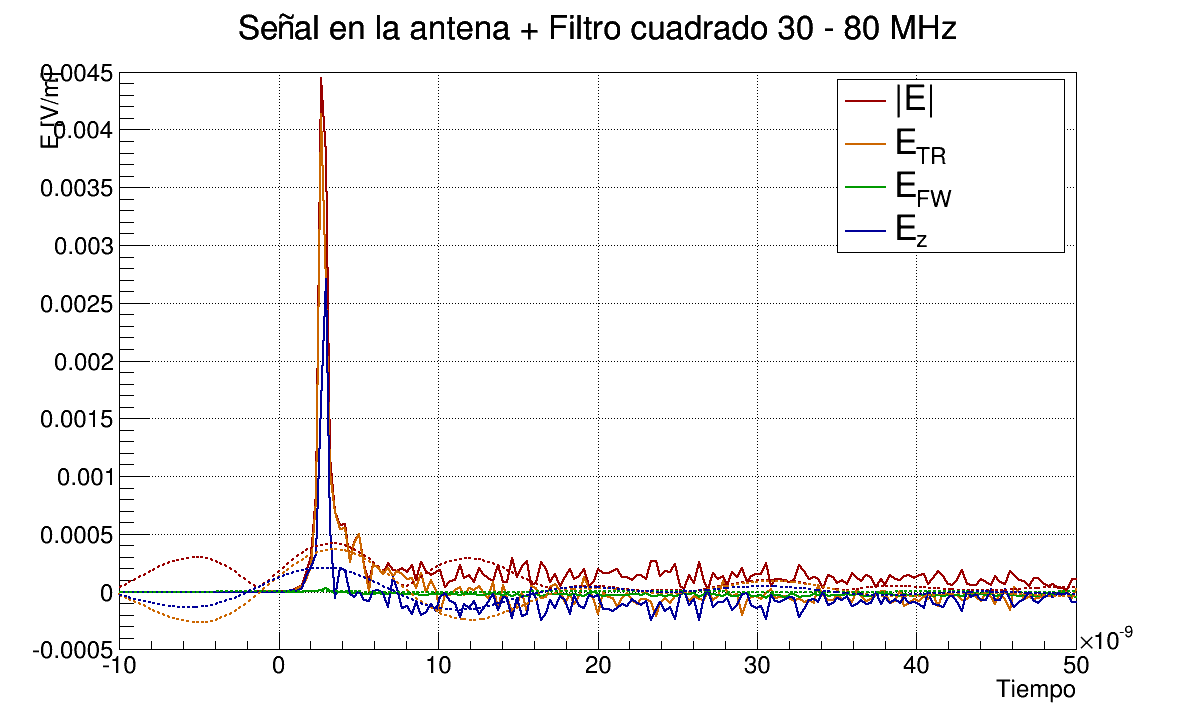
\includegraphics[width=0.8\textwidth]{./fig/simulacionRadio/antennaFilt}
		\caption{\label{fig:antHEnv}
		asd
		}
	\end{figure}
	
\section{Caracterizaci\'on de eventos ES}

Dado que este es el primer trabajo en el que se simula la señal de radio emitida por neutrinos ES, se dedicará esta sección a su caracterización.

	\subsection{Caracter\'isticas generales: evento típico}
	
	Para caracterizar la emisión de radio de una lluvia iniciada por un neutrino ES es buena idea comenzar con un \emph{evento típico}, y luego observar su comportamiento al variar diferentes parámetros.
	En particular, a la hora de definir una lluvia ES será necesario determinar el canal de decaimiento del \tauon{}, la energía transferida a la lluvia $E_v$ y sus parámetros geométricos $(\theta,{\rm x_d},\phi)$.
	Entonces, para el evento típico en este trabajo se eligieron los que se resumen en la tabla \ref{tab:paramTestShower}.
	%
	\begin{table}[ht!]
	 \begin{center}
	  \begin{tabular}{|c|cccc|}
	   \hline
	   Canal de decaimiento & $E_v$ & $\theta$ & \xd{} & $\phi$ \\
	   \hline
	   $\tau\rightarrow e^- \nu_{e^-}\nu\tau$ & \cant{10^{18}}{eV} & \cant{90.5}{^\circ} & \cant{25}{m} & \cant{90}{^\circ} \\
	   \hline
	  \end{tabular}
	  \caption{\label{tab:paramTestShower}
	  Parámetros de simulación del \emph{evento típico} que se utilizará como referencia.
	  }
	 \end{center}
	\end{table}
	%
	La energía visible de una lluvia se refiere a toda la energía que se llevan las partículas no penetrantes, que luego será transferida a la EAS.
	Por ejemplo, en este caso en partícular la lluvia será iniciada por un electrón de \cant{10^{18}}{eV}.
	A diferencia del calculo realizado para Auger, en esta parte del análisis las lluvias ES se caracterizarán por su energía visible $E_v$ y no por la energía del \tauon{} emergente.
	Esto es solo una elección que deberá ser tneida en cuenta a la hora de calcular la exposición del detector.
	
	Dado que el efecto geomagnético contribuye con una parte importante de la señal a nivel del suelo, el resultado de la simulación depende de la ubicación geográfica en la que se realiza, en partícular de su intensidad e inclinación.
	El efecto que eso puede causar en la simulación se trata en la sección \ref{sc:bfield}, pero es importante tener en mente que nuestra lluvia típica se simuló en Malargüe, donde la intensidad del campo es de \cant{0.2414}{Gauss} y tiene una inclinación de $-36.2951^\circ$, es decir, apunta hacia el suelo y el ángulo de su dirección con la normal es de $53.7049^\circ$.
	
	
	
	
	
	\subsubsection{Huella sobre el detector - Cono \cher}
	
	Otra cualidad importante a tener en cuenta es la geometría de la huella que pueden dejar estas lluvias sobre el detector.
	En las figuras \ref{fig:testFootprint_Cone} a \ref{fig:testFootprint_E0z} se grafican las distintas componentes de la se\~nal de radio sobre un arreglo de antenas cuyo paso es \cant{1000}{m} en la dirección de propagación y \cant{100}{m} en la dirección transversal para una lluvia que fue inyectada en el punto $(x,y,z)=(0,0,25){\rm m}$.
	
	La figura \ref{fig:testFootprint_Cone} muestra el módulo del máximo campo eléctrico registrado por cada antena a nivel del suelo.
	%
	\begin{figure}[ht!]
		\centering
		\includegraphics[width=\textwidth]{./fig/simulacionRadio/{foorPrint_Cone_ZWv1.22_ntuples_v1.21_ChTest_phi_90_18_89.5_90_25_1238_E0}.png}
		\caption{\label{fig:testFootprint_Cone}
		Huella de campo eléctrico generada por la lluvia ES típica. En rojo se muestra la zona de impacto del cono \cher{} si el máximo de la lluvia se encuentra a \cant{11}{km} del punto de decaimiento. Esta curva se obtuvo a partir de la ecuación \ref{eq:conewidth}, a la que se llegó mediante hipótesis geométricas.
		}
	\end{figure}
	%
	Hay tres aspectos muy importantes a destacar de esta figura.
	El primero es que, como se observa en línea roja, la zona de impacto del cono \cher{} predicha por la ecuación \ref{eq:conewidth} coincide con la huella de radio de manera notable.
	Para obtener la predicción se utilizaron los parámetros de la simulación para la altura de decaimiento y el ángulo cenital, mientras que la posición del máximo de la lluvia se obtuvo mediante prueba y error, pero utilizando valores razonables\footnote{Para una lluvia de \cant{10^{18}}{eV} el máximo de la lluvia ronda los \cant{10}{km}}.
	Si bien \zhs{} realiza la simulación microscópicamente, es decir, sin realizar ninguna suposición sobre los mecanismos de emisión, se nota que los resultados obtenidos pueden ser descriptos a orden cero a partir de razonamientos meramente geométricos (ver sección \ref{sbsc:geom_emision}).
	
	La segunda observación es que en al dirección de propagación de la lluvia la huella alcanza niveles detectables ($>\sim100{\rm \mu V/m}$) durante aproximadamente \cant{50}{km}.
	Esta es una cualidad muy favorable a la hora detectar este tipo de eventos, ya que aumenta la probabilidad de disparar antenas.
	Por último, en contraposición a lo anterior, en la dirección transversal a la de propagación el tamaño de la huella es de al rededor de \cant{2}{km}, es decir, las lluvias ES generan huellas muy alargadas sobre el detector.
	Esta es la característica fundamental a partir de la cual se pueden distinguír neutrinos ES. 
	Ya que los eventos inclinados que podrían generar su background se desarrollan muy alto en la atmósfera, generarán huellas cuyo largo será similar al de las lluvias ES, pero con un ancho mucho mayor.
	Esta última conclusión se infiere de que, al ubicarse el máximo de la lluvia más alto en la atmósfera, la apertura del cono al alcanzar el suelo será mucho mayor.
	Este tema se volverá a abordar con mayor detalle en la sección \ref{REF}.
	
	\subsection{Polarización de la señal - Influencia del campo magn\'etico terrestre}
	
	También es interesante analizar las componentes del camponentes del campo eléctrico de la huella.
	En la figura \ref{fig:malField} se muestran las contribuciones al campo eléctrico a nivel del suelo para una lluvia completamente horizontal ($\theta=90^\circ$) y que se desplaza de Oeste a Este ($\phi=90^\circ$).
	%
	\begin{figure}[ht!]
		\centering
		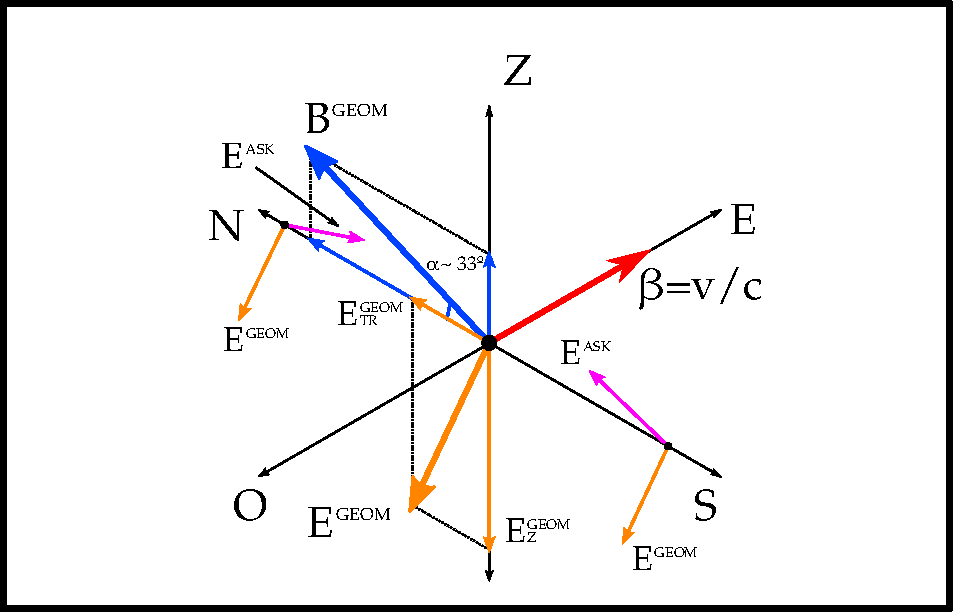
\includegraphics[width=0.8\textwidth]{./fig/simulacionRadio/malField}
		\caption{\label{fig:malField}
		Esquema de las componentes del campo elctrico para una lluvia que se desplaza de Oeste a Este en Malargüe. Se considerarán los campos hacia arriba, o la componente $z$, y el campo transversal a la dirección de propagación de la lluvia sobre el suelo, componente ${\rm TR}$. Se desprecia por el momento la componente ${\rm FW}$, tambien sobre el suelo pero en la dirección de propagación. La contribución geomagnética conserva su dirección (transversal y hacia arriba) en todo el suelo. Por otro lado, el aporte del efecto Askaryan tiene una componentes transversales opuestas en el sector norte y el sur, mientras que la componente $z$ siempre es positiva.
		}
	\end{figure}
	%
	Por simplicidad es conveniente pensar en el campo en el sistema de referencia definido por la coordenada $z$ y las direcciónes paralela (${\rm FW}$) y transversal (${\rm TR}$) a la dirección de propagación sobre el suelo.
	Desde esta persectiva, a primer orden la contribución geomagnética al campo eléctrico tiene dirección $({\rm TR},z)$ ya que por construcción es perpendicular a la dirección de propagación.
	Por otro lado, a cada lado del eje de la lluvia la componente Askaryan tiene direcciones opuestas pero sobre el suelo siempre posee componente en $z>0$.
	
	En las figuras \ref{fig:testFootprint_E0tr} y \ref{fig:testFootprint_E0z} se grafican el campo en dirección ${\rm TR}$ y en dirección $z$ de la huella de la lluvia.
	%
	\begin{figure}[ht!]
		\centering
		\includegraphics[width=\textwidth]{./fig/simulacionRadio/{foorPrint_ZWv1.22_ntuples_v1.21_ChTest_phi_90_18_89.5_90_25_1238_E0x}.png}
		\caption{\label{fig:testFootprint_E0tr}
		Huella de campo eléctrico en la dirección ${\rm TR}$. La intensidad del cono \cher{} es distinta a ambos lados del eje de la lluvia.
		Cuando la coordenada transversal es positiva el efecto Askaryan y el geomagnético se suprimen mientras que cuando es negativa se favorecen.
		}
	\end{figure}
	%
	Como puede observarse en la figura \ref{fig:testFootprint_E0tr}, la intensidad del cono \cher{} no es simétrica respecto del eje de la lluvia.
	Esto se debe a que, como se esquematizó en la figura \ref{fig:malField}, de un lado del mismo las contribuciones Askaryan y geomagnética en la dirección ${\rm TR}$ se suprimen mientras que del otro se favorecen.
	%
	\begin{figure}[ht!]
		\centering
		\includegraphics[width=\textwidth]{./fig/simulacionRadio/{foorPrint_ZWv1.22_ntuples_v1.21_ChTest_phi_90_18_89.5_90_25_1238_E0z}.png}
		\caption{\label{fig:testFootprint_E0z}
		Huella de campo eléctrico en la dirección $z$. En esta dirección las contribuciones geomagnética y Askaryan se suman en cualquier punto del suelo.
		}
	\end{figure}
	%
	Por otro lado, si se considera la componente $z$ del campo de ambas contribuciones no presenta ningun cambio de signo en el plano del suelo.
	Por esta razon la figura \ref{fig:testFootprint_E0z} presenta una huella mucho más simétrica.
	
	Por ultimo, hasta el momento se despreció la componente ${\rm FW}$. 
	Dado que las lluvias ES son casi horizontales la aparición de esta componente a nivel del suelo se vuelve despreciable, como se observa en la figura \ref{fig:testFootprint_E0fw} si se compara la intensidad de campo de la huella con la de las figuras \ref{fig:testFootprint_E0tr} y \ref{fig:testFootprint_E0z}.
	%
	\begin{figure}[ht!]
		\centering
		\includegraphics[width=\textwidth]{./fig/simulacionRadio/{foorPrint_ZWv1.22_ntuples_v1.21_ChTest_phi_90_18_89.5_90_25_1238_E0y}.png}
		\caption{\label{fig:testFootprint_E0fw}
		Campo eléctrico en la dirección ${\rm FW}$. Su intensidad es despreciable si se la compara con la de las direcciones ${\rm TR}$ y $z$.
		}
	\end{figure}
	
% 	\clearpage
	
	
% 	\begin{figure}[ht!]
% 		\centering
% 		\includegraphics[width=\textwidth]{./fig/simulacionRadio/{foorPrint_ZWv1.22_ntuples_v1.22_ChTest_phi_90_18_89.5_90_25_1238_E}.png}
% 		\includegraphics[width=\textwidth]{./fig/simulacionRadio/{foorPrint_ZWv1.22_ntuples_v1.22_ChTest_phi_90_18_89.5_90_25_1238_E0}.png}
% 		\caption{\label{fig:footprint_E_HEnv}
% 		asd
% 		}
% 	\end{figure}
% 	
% 	\begin{figure}[ht!]
% 		\centering
% 		\includegraphics[width=\textwidth]{./fig/simulacionRadio/{foorPrint_ZWv1.22_ntuples_v1.22_ChTest_phi_90_18_89.5_90_25_1238_EHB}.png}
% 		\includegraphics[width=\textwidth]{./fig/simulacionRadio/{foorPrint_ZWv1.22_ntuples_v1.22_ChTest_phi_90_18_89.5_90_25_1238_ELB}.png}
% 		\caption{\label{fig:footprint_HB-LB_HEnv}
% 		asd
% 		}
% 	\end{figure}
% 	
% 	\begin{figure}[ht!]
% 		\centering
% 		\includegraphics[width=\textwidth]{./fig/simulacionRadio/{foorPrint_ZWv1.22_ntuples_v1.22_ChTest_phi_90_18_89.5_90_25_1238_E}.png}
% 		\includegraphics[width=\textwidth]{./fig/simulacionRadio/{foorPrint_ZWv1.22_ntuples_v1.22_ChTest_phi_90_18_89.5_90_25_1238_E0}.png}
% 		\caption{\label{fig:footprint_E_HEnv}
% 		asd
% 		}
% 	\end{figure}
% 	
% 	\clearpage
	
	\begin{figure}[ht!]
		\centering
		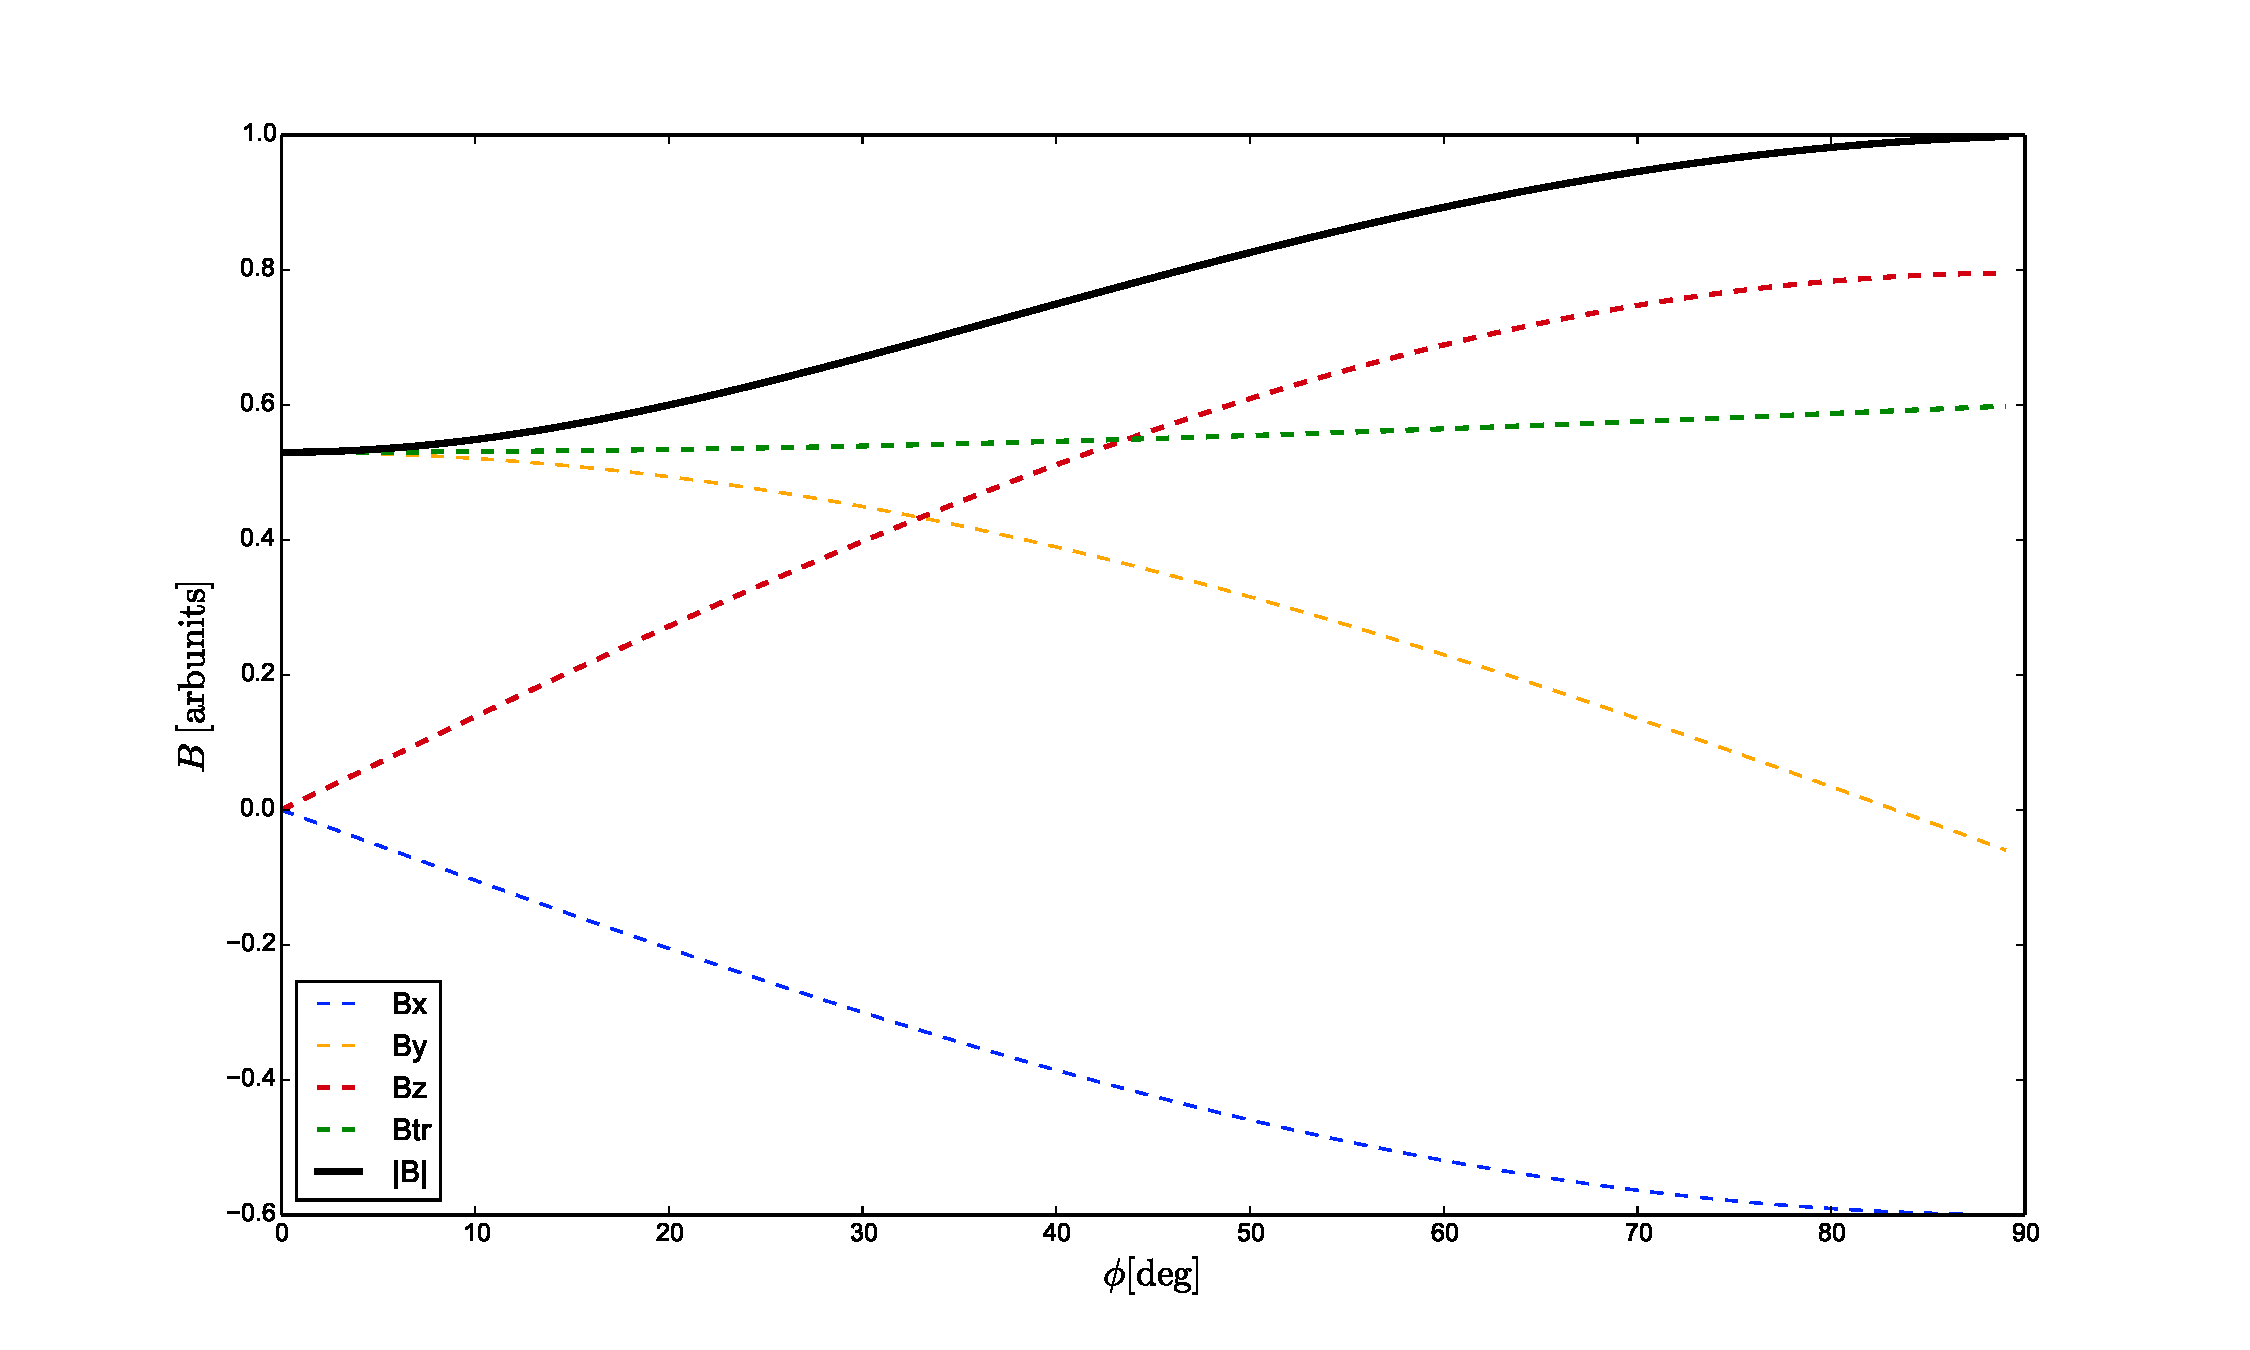
\includegraphics[width=\textwidth]{./fig/EASRadio/geomComps_Malarge}
		\caption{\label{fig:geomComps_Malarge}
		asd
		}
	\end{figure}
	
	\begin{figure}[ht!]
		\centering
		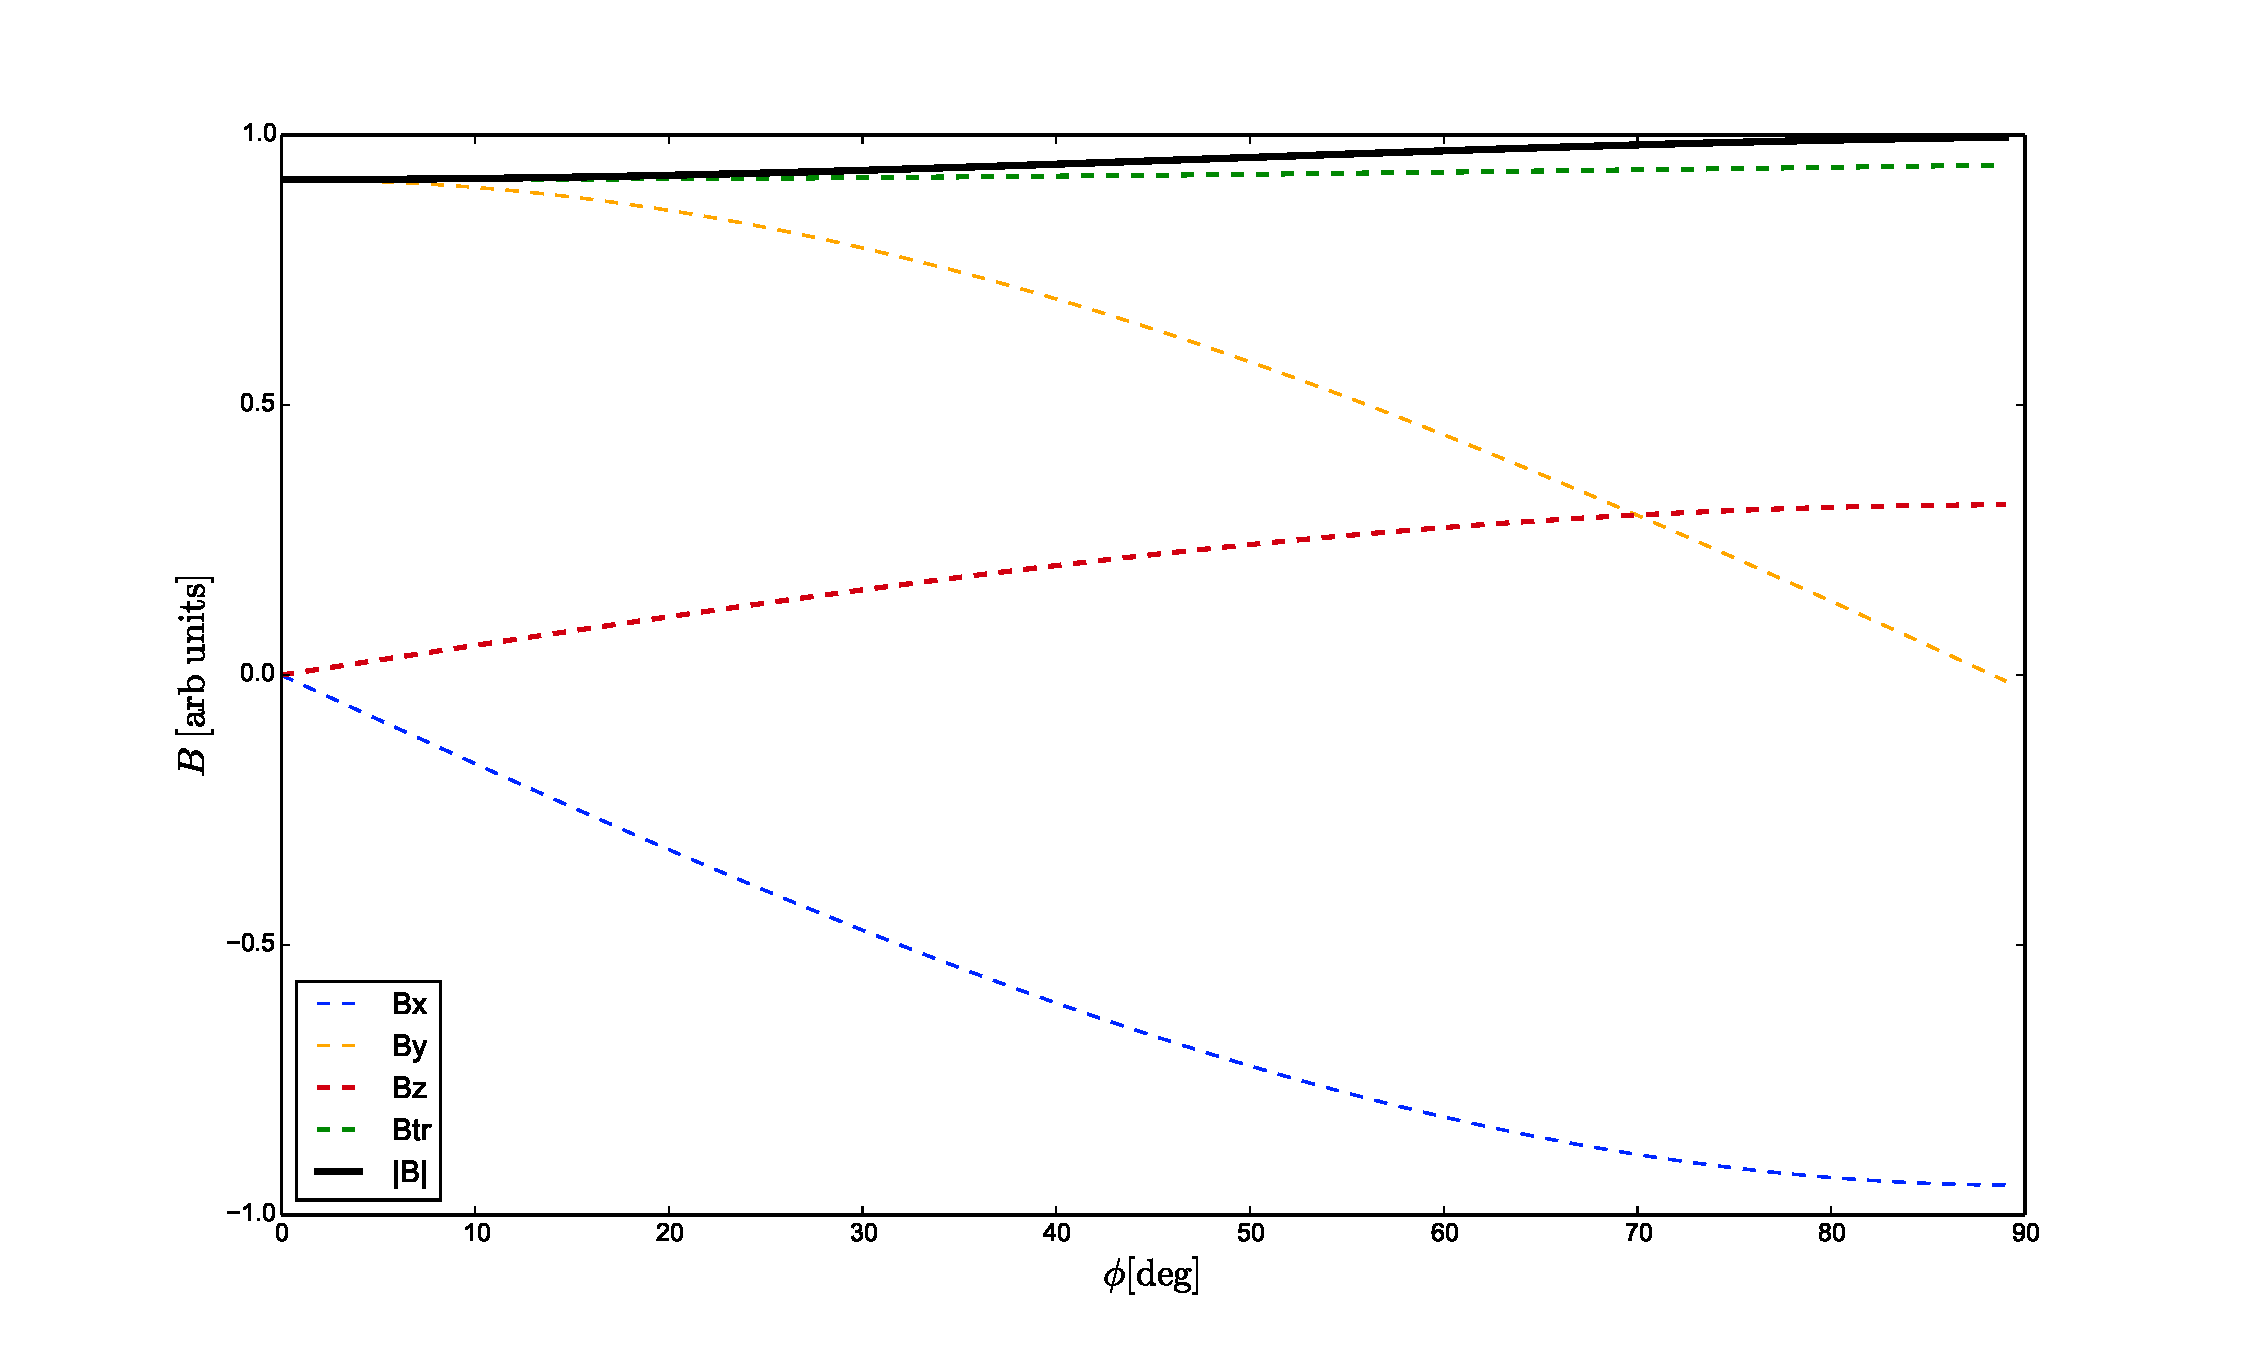
\includegraphics[width=\textwidth]{./fig/EASRadio/geomComps_Tunka}
		\caption{\label{fig:geomComps_Tunka}
		asd
		}
	\end{figure}
	
	\begin{figure}[ht!]
		\centering
		\includegraphics[width=\textwidth]{./fig/simulacionRadio/{ZHSEvent_18_89.5_0_25_On_1238_E}.png}
		\includegraphics[width=\textwidth]{./fig/simulacionRadio/{ZHSEvent_18_89.5_0_25_Off_1238_E}.png}
		\caption{\label{fig:testFootprint_Ez}
		asd
		}
	\end{figure}
	
	\begin{figure}[ht!]
		\centering
		\includegraphics[width=\textwidth]{./fig/simulacionRadio/{ZHSEvent_18_89.5_0_25_On_1238_Ey}.png}
		\includegraphics[width=\textwidth]{./fig/simulacionRadio/{ZHSEvent_18_89.5_0_25_Off_1238_Ey}.png}
		\caption{\label{fig:testFootprint_Ez}
		asd
		}
	\end{figure}
	
	\begin{figure}[ht!]
		\centering
		\includegraphics[width=\textwidth]{./fig/simulacionRadio/{ZHSEvent_18_89.5_0_25_On_1238_Ez}.png}
		\includegraphics[width=\textwidth]{./fig/simulacionRadio/{ZHSEvent_18_89.5_0_25_Off_1238_Ez}.png}
		\caption{\label{fig:testFootprint_Ez}
		asd
		}
	\end{figure}
	
		\begin{figure}[ht!]
		\centering
		\includegraphics[width=\textwidth]{./fig/simulacionRadio/{ZHSEvent_18_89.5_0_25_On_1238_Ex}.png}
		\includegraphics[width=\textwidth]{./fig/simulacionRadio/{ZHSEvent_18_89.5_0_25_Off_1238_Ex}.png}
		\caption{\label{fig:testFootprint_Ez}
		asd
		}
	\end{figure}
	
	Bon y Boff
	
	mostrar que los efectos son comparables.
	
	velocidad de drift peque\~na por alra densidad en la atmósfera.
	
	
% 	\subsection{Evoluci\'on de la se\~nal a nivel del suelo}
% 		
% 	
% 	mostrar evolucion del EMax a lo largo de la lluvia
% 	
% 	mostrar espectro y evolucion
% 	
% 	mostrar fit del maximo de la lluvia como funcion de xd y theta y dependencia con la energia
% 	
% 		\subsubsection{Evoluci\'on de la polarizaci\'on}
% 		
% 		cambio askaryan geomagnetico?
	
	\subsection{Corte en $\theta$}
	
	plots dado xd para diferentes thetas
	mostrar tomataso
	
	\clearpage
	\clearpage
	\subsection{Distribuci\'on de part\'iculas vs. se\~nal de radio}
	
	remarcar que el footprint es mucho mas extenso que la distribucion de particulas
	
	\begin{figure}[ht!]
		\centering
		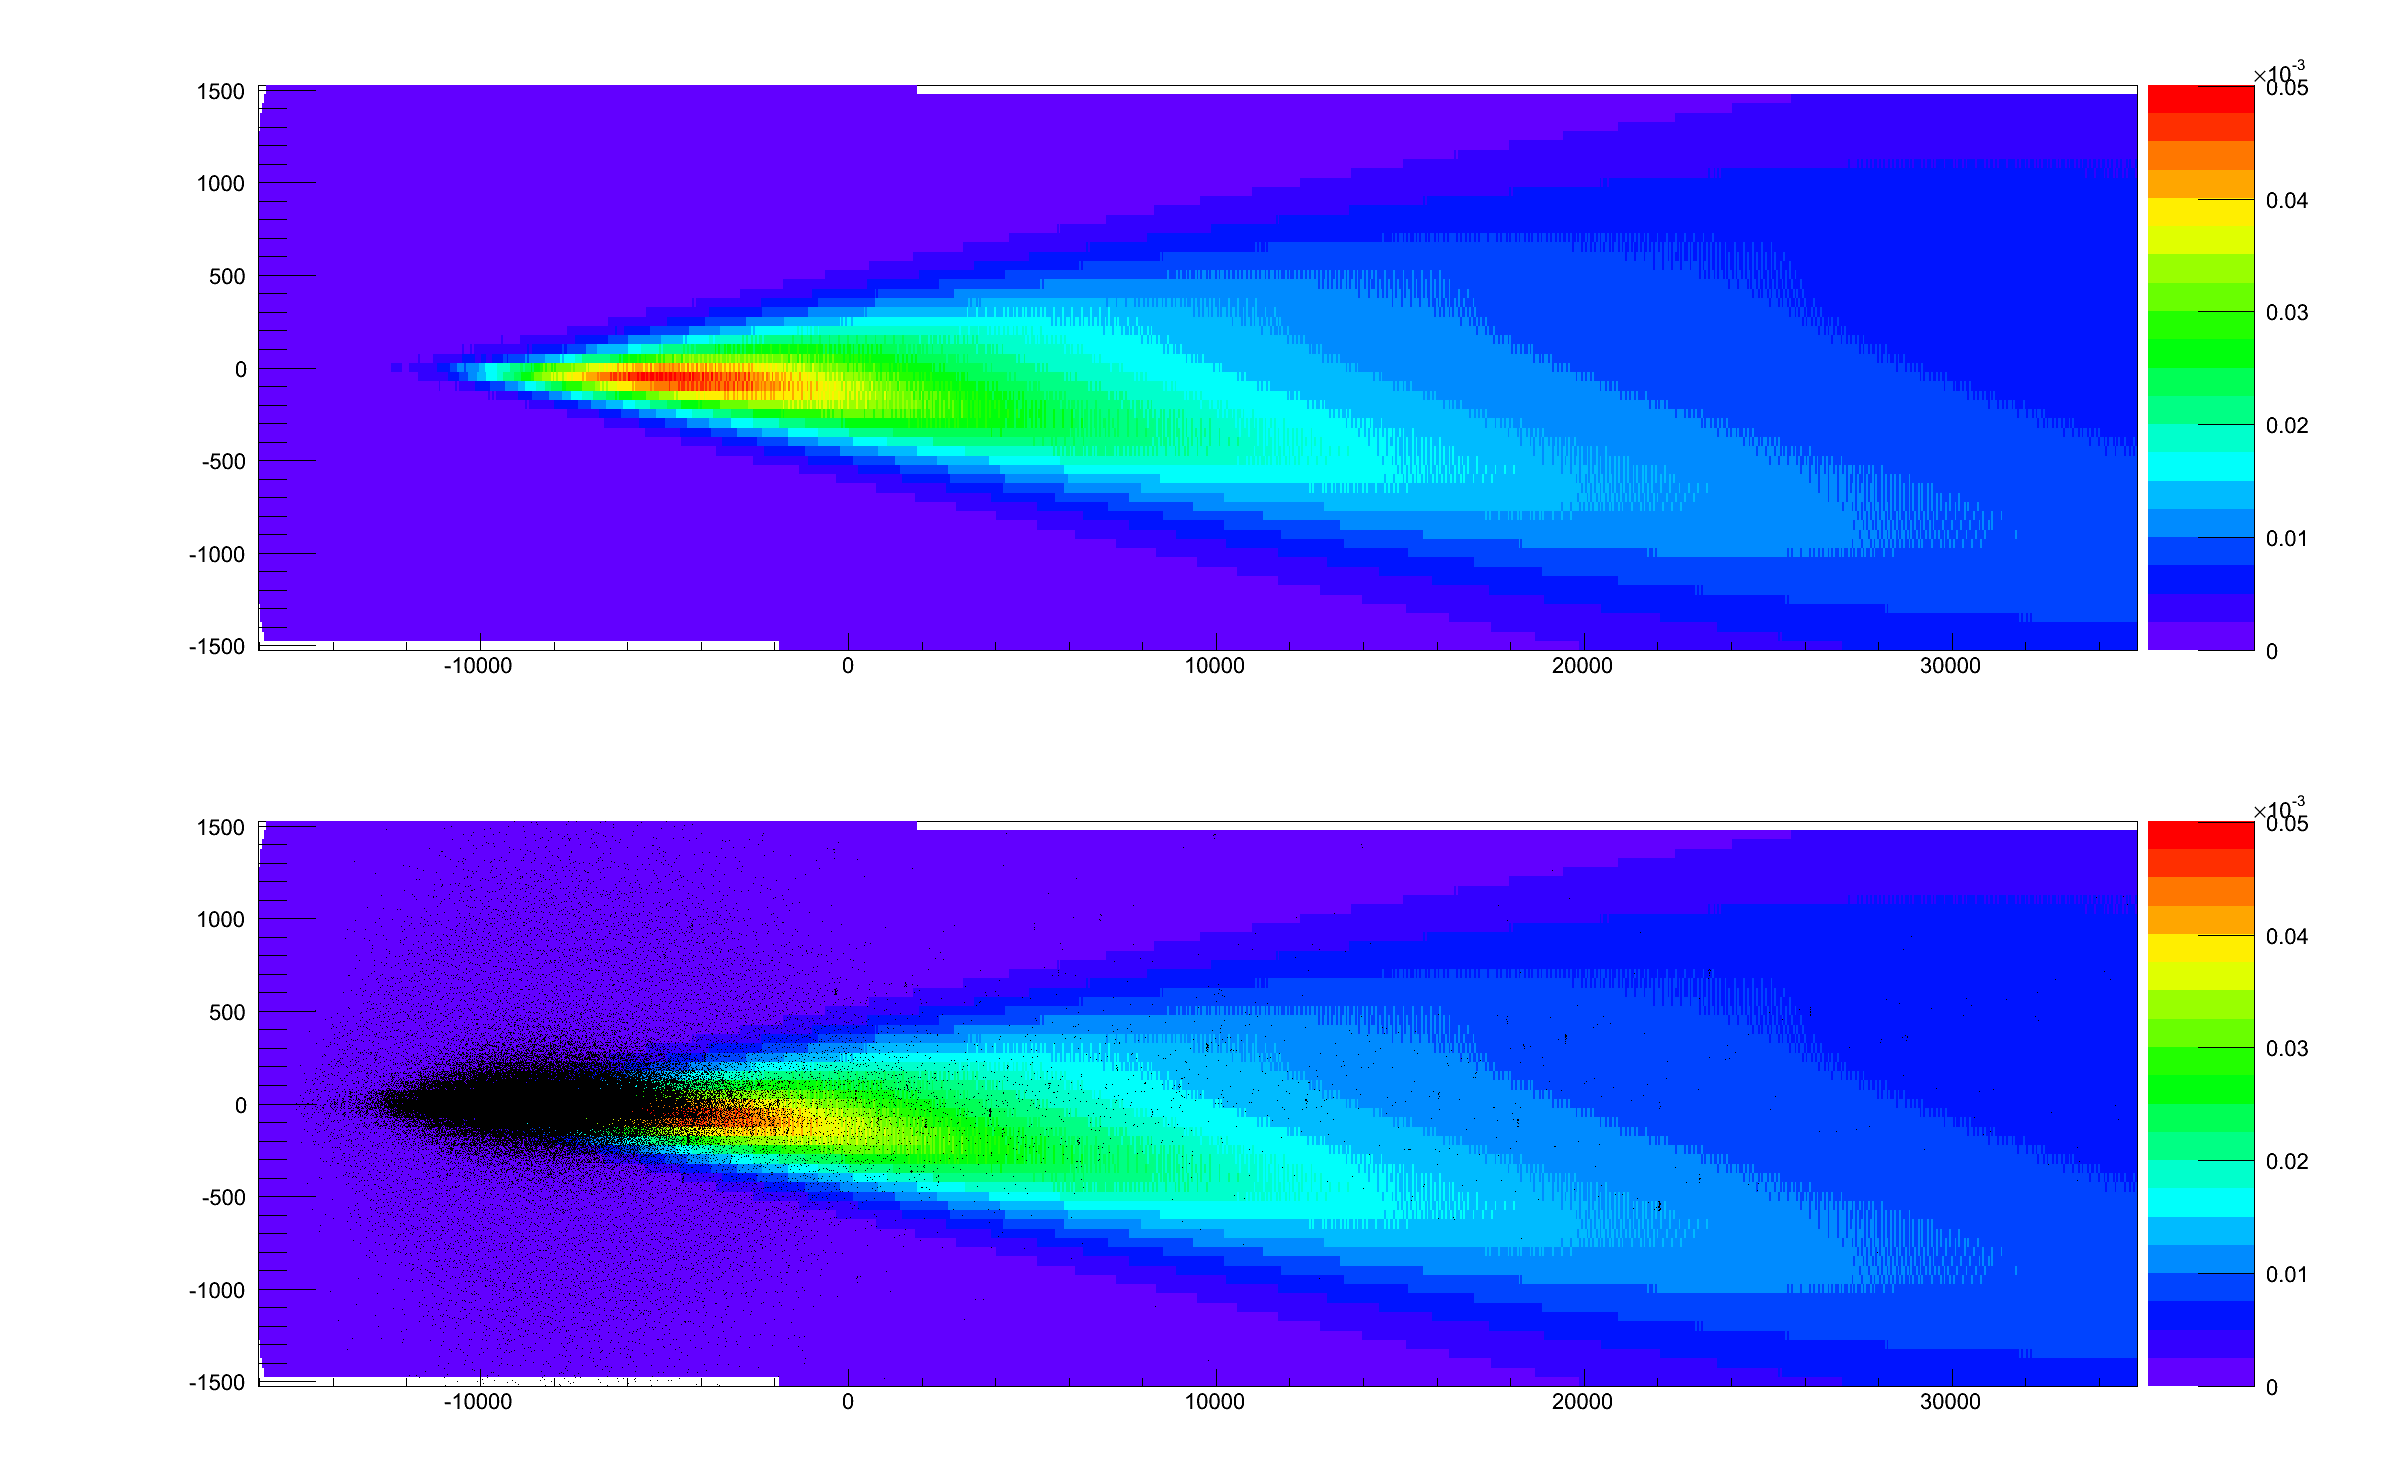
\includegraphics[width=\textwidth]{./fig/simulacionRadio/ZHSEvent_1238_denseArray_E_Particulas}
		\caption{\label{fig:sim_foot_y_part}
		asd
		}
	\end{figure}
	
	\subsection{Dependencia con el canal de decaimiento del \tauon{}}
	
	
	
	\begin{figure}[ht!]
		\centering
		\includegraphics[width=\textwidth]{./fig/simulacionRadio/{showerWidth_ZWv1.43_ntuples_v1.22_Channels_All}.pdf}
		\caption{\label{fig:showerWidth}
		asd
		}
	\end{figure}
	
	\begin{figure}[ht!]
		\centering
		\includegraphics[width=\textwidth]{./fig/simulacionRadio/{showerMaxE_ZWv1.43_ntuples_v1.22_Channels_All}.pdf}
		\caption{\label{fig:showerMaxE}
		asd
		}
	\end{figure}
	
	\begin{figure}[ht!]
		\centering
		\includegraphics[width=\textwidth]{./fig/simulacionRadio/{showerArea_ZWv1.43_ntuples_v1.22_Channels_All}.pdf}
		\caption{\label{fig:showerArea}
		asd
		}
	\end{figure}
	Graficar distribuciones de diferentes variables que importen para diferentes canales.
	
	Energia visible
	Ancho de la lluvia
	Maximo del footprint
	
	
	

